

%!TEX root = ../Notes.tex
\section{Loops and the Fundamental Group} We have shown that the product of two path homotopy classes is well defined. For the purposes of defining a group of path homotopy classes, we would like a set of paths whose products have the same endpoints as the original paths. This simplification motivates the two definitions which follow: 
\begin{definition}
	Let $f$ be a path in $X$ such that $f(0) = f(1) = x_0\in X$. Then $f$ is a \textbf{loop} in $X$ based at $x_0$. 
\end{definition}

Note that if $f,g$ are loops in $X$ based at some point $x_0\in X$, then their product $f*g$ is also a loop based at $x_0$. In particular, we then have that $[f],[g]$ and $[f][g] = [f*g]$ are all path-homotopic classes of loops based at $x_0$. 
\begin{definition}
	Let $(X,F_x)$ be a topological space, and let $x_0\in X$. 
	
	Define $\pi_1(X,x_0)$ as the set of path homotopy classes of loops based at $x_0$ endowed with the product of path homotopy classes. We call $\pi_1(X,x_0)$ the \textbf{fundamental group of $X$ based at $x_0$}. 
\end{definition}

\subsection{The Fundamental Group is a Group}

Our ultimate goal is to harness the power of group theory from abstract algebra to study topological spaces. We defined the fundamental group of $X$ based at $x_0$ with the path homotopy class product operation. Naturally, we would like to prove that $\pi_1(X,x_0)$ endowed with the product operation is actually a group. In other words, if $(X,F_x)$ is a topological space with $x_0\in X$, we must prove the following: 
\begin{enumerate}
	\item $\pi_1(X,x_0)$ is closed under the operation $[][]$. In other words, for $[f],[g]\in \pi_1(X,x_0)$, $[f][g] \in \pi_1(X,x_0)$. 
	\item The operation $[][]$ is associative. In other words, given $[f],[g],[h]\in \pi_1(X,x_0)$:
	\[ ([f][g])[h] = [f]([g][h])\]
	\item $\pi_1(X,x_0)$ contains an identity element. In other words, there exists $[e]\in \pi_1(X,x_0)$ such that for all $[f]\in\pi_1(X,x_0)$:
	\[[e][f] = [f][e] = [f]\]
	\item Every element of $\pi_1(X,x_0)$ has an inverse. In other words, given $f\in \pi_1(X,x_0)$, there exists $g\in \pi_1(X,x_0)$ such that:
	\[[f][g] = [g][f] = [e]\]
\end{enumerate}

If $\pi_1(X,x_0)$ satisfies all of these requirements, $\pi_1(X,x_0)$ is a group. 
\begin{lemma}
	[Closure] Let $(X,F_x)$ be a topological space, and let $x_0\in X$. Let $[f],[g]\in \pi_1(X,x_0)$. Then:
	\[[f][g] \in \pi_1(X,x_0)\]
\end{lemma}
\begin{proof}
	We see that:
	\[[f][g] = [f*g]\]
	We know by a previous result that $f*g$ is a path in $X$ from $x_0$ to $x_0$ since $x_0$ is both the starting point of $[f]$ and the endpoint of $[g]$. Consequently, $f*g$ is a loop in $X$ based at $x_0$, so $[f*g] \in \pi_1(X,x_0)$. 
\end{proof}

Next, we will show that path homotopy path products of loops based at a point are associative. 
\begin{lemma}
	[Associativity] Let $(X,F_x)$ be a topological space, and let $x_0\in X$. Let $[f],[g],[h]\in \pi_1(X,x_0)$. Then:
	\[ ([f][g])[h] = [f]([g][h])\]
\end{lemma}
\begin{proof}
	Before actually proving the result, we will explicitly write the formulas for $(f*g)*h$ and $f*(g*h)$:
	\[(f*g)*h = 
	\begin{cases}
		f(4s) & s\in [0,\frac14] \\
		g(4s-1) & s\in[\frac14,\frac12] \\
		h(2s-1) & s\in [\frac12,1] 
	\end{cases}
	\qquad\qquad f*(g*h) = 
	\begin{cases}
		f(2s) & s\in [0,\frac12] \\
		g(4s-2) & s\in[\frac12,\frac34] \\
		h(4s-3) & s\in [\frac34,1] 
	\end{cases}
	\]
	
	We need to construct a homotopy from $(f*g)*h$ to $f*(h*g)$.
	\[ 
	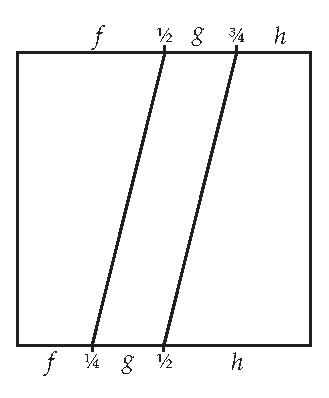
\includegraphics[width=150pt]{images/fundamental_group/fgh_diagram} \]
	
	Based on our formulas for $(f*g)*h$ and $f*(g*h)$, we parameterize the function $F:I\times I \to X$ by:
	\[F(s,t) = 
	\begin{cases}
		f\left(\frac{4s}{1+t} \right)& s \in \left[ 0,\frac{1+t}4 \right] \\
		g(4s-1-t) & s\in \left[\frac{1+t}4, \frac{2+t}4\right] \\
		h\left(\frac{4s}{2-t} - \frac{2+t}{2-t} \right) & s\in \left[\frac{2+t}4,1\right] 
	\end{cases}
	\]
	
	We claim and will verify that $F$ is a homotopy from $(f*g)*h$ to $f*(g*h)$. We first prove continuity using the pasting lemma as usual. The proof that each of the piecewise parts of $F$ is defined on a closed set is left as a (relatively trivial but tedious) exercise.
	
	We will, however, show that on the boundaries between these regions, the piecewise parts agree. We see: 
	\begin{eqnarray*}
		f\left(\frac{4}{1+t} \cdot \left(\frac{1+t}4\right)\right) & = & f(1) = x_0 \\
		g\left(4\cdot\left(\frac{1+t}4\right)-1-t\right) & = & g(0) = x_0\\
		g\left(4\cdot\left(\frac{2+t}4\right)-1-t\right) & = & g(1) = x_0\\
		h\left(\frac{4}{2-t} \cdot \left(\frac{2+t}4\right)- \frac{2+t}{2-t}\right) & = & h(0) = x_0\\
	\end{eqnarray*}
	so continuity follows by the pasting lemma. Note that we assume $f,g,h$ are continuous so that things like $h\left(\frac{4s}{2-t} - \frac{2+t}{2-t} \right)$ are because compositions of continuous functions are continuous and over $t\in I$, $\frac{4s}{2-t} - \frac{2+t}{2-t}$ is continuous. The justification is similar for the other piecewise parts in the definition of $F$. 
	
	We now verify that $F$ gives a path from $x_0$ to $x_0$ for every fixed $t\in I$. We see that: 
	\begin{eqnarray*}
		F(0,t) & = & f(0) = x_0\\
		F(1,t) & = & h(1) = x_0\\
	\end{eqnarray*}
	as desired.
	
	Finally, we need to show that $F$ provides a homotopy from $(f*g)*h$ to $f*(g*h)$. We have that:
	\[F(s,0) = 
	\begin{cases}
		f\left(4s \right)& s \in \left[ 0,\frac{1+t}4 \right] \\
		g(4s-1) & s\in \left[\frac{1+t}4, \frac{2+t}4\right] \\
		h\left(2s - 1 \right) & s\in \left[\frac{2+t}4,1\right] 
	\end{cases}
	\qquad = \qquad (f*g)*h \]
	\[F(s,1) = 
	\begin{cases}
		f\left(2s \right)& s \in \left[ 0,\frac{1+t}4 \right] \\
		g(4s-2) & s\in \left[\frac{1+t}4, \frac{2+t}4\right] \\
		h\left(4s - 3 \right) & s\in \left[\frac{2+t}4,1\right] 
	\end{cases}
	\qquad = \qquad f* (g*h)\]
	as desired, so $F$ satisfies the three properties of a homotopy from $(f*g)*h$ to $f*(g*h)$.
	
	We have constructed $F(s,t)$ such that $F$ is a homotopy from $(f*g)*h$ to $f*(g*h)$ which implies that $(f*g)*h \sim f*(g*h) \Rightarrow [(f*g)*h] = [f*(g*h)]$. It immediately follows that
	\[ ([f][g])[h] = [f]([g][h])\]
\end{proof}
\begin{lemma}
	[Identity] Let $f$ be a path in $X$ which begins at $x_0$ and ends at $x_1$. Then $f*e_{x_1}\sim f$ and $e_{x_0}* f \sim f$. \footnote{Recall that $\sim$ denotes ``path homotopy."} 
\end{lemma}
\begin{proof}
	We prove that $f* e_{x_1}\sim f$. The other case is similar.
	
	In order to define a homotopy, at $t$, we will ``do'' $f$ for $s\in [0,t(1)+(1-t)\tfrac{1}{2}]$ or, by simplification, $s\in[0,\tfrac{t+1}{2}]$ and $e_{x_1}(t)$ for $s\in [\tfrac{t+1}{2},1]$.
	
	Define $F:I\times I \to X$ by
	\[F(s,t)= 
	\begin{cases}
		f\left(\tfrac{2s}{t+1}\right) & s\in \left[0,\tfrac{t+1}{2}\right] \\\
		e_{x_1} & s\in \left[\frac{t+1}{2},1\right] 
	\end{cases}
	\]
	
	This is: 
	\begin{itemize}
		\item[Continuous:] By the Pasting lemma, as $f, e_{x_1}$ are continuous on closed domains it suffices to check that they agree for $s=\tfrac{t+1}{2}$. This follows easily, as $f\left(\frac{2\tfrac{t+1}{2}}{t+1}\right)=f(1)=x_1$, and $e_{x_1}\left(\tfrac{t+1}{2}\right)=x_1$. 
		\item[A homotopy:]
		\[F(s,0)= 
		\begin{cases}
			f(2s) & s\in\left[0,\tfrac{1}{2}\right]\\
			e_{x_1}(t) & s\in\left[\tfrac{1}{2},1\right] 
		\end{cases}
		= f*e_{x_1}\]
		and
		\[F(s,1)= 
		\begin{cases}
			f(s) & s\in [0,1]\\
			e_{x_1} & s\in [1,1]=f. 
		\end{cases}
		\]
		\item[ A path: ] $F(0,t)=f(0)=x_0$, and $F(1,t)=e_{x_1}=x_1$, hence $F$ is a path. 
	\end{itemize}
	Thus $f*e_{x_1}\sim f$. 
\end{proof}

We've now shown that $\pi_1(X, x_0)$ is closed, has an identity, and the operation is associative, so just showing that inverses exist proves that it's a group. 
\begin{lemma}
	[Inverses] Let $f$ be a path in $X$ from $x_0$ to $x_1$. Then $f*\overline{f}\sim e_{x_0}$ and $\overline{f}*f\sim e_{x_0}$. 
\end{lemma}

The ``wrong" approach: increase the speed over $f$ and $\overline{f}$ and wait at $x_1$. The ``right" approach: travel successively smaller distances along $f$. 
\begin{proof}
	We show only that $f*\overline{f}\sim e_{x_0}$, and the other case follows similarly.
	
	Define $F:I\times I\to X$ by
	\[ F(s,t)= 
	\begin{cases}
		f(2s) & s\in \left[0,\tfrac{1-t}{2}\right] \\
		f(1-t) & s\in \left[\tfrac{1-t}{2},\tfrac{1+t}{2}\right]\\
		\overline{f}(2s-1) & s\in\left[\tfrac{1+t}{2}, 1\right] 
	\end{cases}
	\]
	This is: 
	\begin{itemize}
		\item[Continuous:] Using the pasting lemma, it suffices to check that these functions agree on their (shared) endpoints. As $f(2(\tfrac{1-t}{2}))=f(1-t)$, and $f(2(\tfrac{1+t}{2})-1)=\overline{f}(t)=f(1-t)$, we conclude that $F$ is continuous.
		
		\item[A homotopy:] Let $t=0$,
		\[F(s,0)= 
		\begin{cases}
			f(2s) & s\in [0,1/2]\\
			f(1) & s\in [1/2,1/2] \\
			\overline{f}(2s-1) & s\in [1/2,1] 
		\end{cases}
		=f*\overline{f}(s)\]
		
		For $t=1$,
		\[F(s,1)= 
		\begin{cases}
			f(2s) & s\in [0,0]\\
			f(0) & s\in [0,1]\\
			\overline{f}(2s-1) & s\in [1,1] 
		\end{cases}
		=e_{x_0}.\]
		
		\item[A path:] For $s=0$, $F(0,t)=f(0)=x_0$. And for $s=1$, $F(1,t)=\overline{f}(1)=x_0$. 
	\end{itemize}
	
	For each loop $f$ based at $x_0$, $\overline{f}$ is a loop based at $x_0$. Thus we have shown closure under inverses. 
\end{proof}

It follows that the action $*$ defines a group on the set of loops based at $x_0$.

Observe that the set of paths does not have a group structure, as there is no definition of multiplication between arbitrary paths. 
\begin{example}
	Let $X=\R^n$ and $x_0$ be a point in $X$. Then $\pi_1(X,x_0)=\langle [e_{x_0}]\rangle$. 
\end{example}

The following theorem relates the fundamental group at a point within a path component to the fundamental group of that point in the ambient space: 
\begin{theorem}
	Let $A$ be a path component of a topological space $X$, and let $x_0\in A$. Then:
	\[\pi_1(A,x_0)\cong \pi_1(X,x_0)\]
	(Note that $\cong$ denotes a group isomorphism and not a homeomorphism) 
\end{theorem}

Before proving the theorem, we will cover two quick non-examples of cases where the theorem could break down.

Recall the circle $S^1$ which we can consider as a subspace of $\R^2$. Since $\R^2$ is a simply connected space, the fundamental group at every point is trivial. On the other hand, picking some point $x_0\in S^1$, the loop around the circle cannot be deformed in $S^1$ to the point $x_0$, so $\pi_1(S^1,x_0)$ is non-trivial and hence not isomorphic to $\pi_1(\R^2,x_0)$ if we embed $S^1$ in $\R^2$. The following picture illustrates $S^1$ with the point $x_0$: 
\begin{center}
	\begin{picture}
		(50,50) \put(0,20){\circle*{3}} \put(0,25){$x_0$} \put(0,0){\circle{100}} 
	\end{picture}
	\vspace{10mm} 
\end{center}

This may seem like a counterexample to the theorem, but in $\R^2$, $S^1$ is not a distinct path component of $\R^2$, so the theorem does not apply. Intuitively, by embedding $S^1$ in $\R^2$, the interior of the circle is part of $\R^2$, so we can deform a loop around $S^1$ based at $x_0$ to the trivial loop by ``pulling'' the loop through the middle of the circle, which we could not do when $S^1$ was considered as a space in its own right.

Consider the following diagram: 
\begin{center}
	\begin{picture}
		(50,50) \put(0,20){\circle*{3}} \put(0,25){$x_0$} \put(0,0){\circle{100}} \put(45,0){\circle*{10}} \put(50,5){A} \put(-45,0){\circle*{10}} \put(-53,5){B} 
	\end{picture}
	\vspace{10mm} 
\end{center}
where we have the space $\R^2$ with $A,B$ removed, so loops based at $x_0$ that run around $A,B$ cannot be deformed into the trivial loop. However, when we consider this space embedded in $\R^2$ as a subspace, it is not an entire path component in $\R^2$, so our theorem does not apply. 

We now prove the theorem: 
\begin{proof}
	Define $\varphi:\pi_1(A,x_0)\to \pi_1(X,x_0)$ by:
	\[\varphi([f]_A) = [f]_X\]
	We claim that $\varphi$ is a \emph{group isomorphism}, i.e. that $\varphi$ is a bijection and a group homomorphism. In other words, we need to show that $\varphi$ is injective, surjective and that if $a,b\in\pi_1(A,x_0)$, then $\varphi(ab) = \varphi(a)\varphi(b)$. For those who have not had algebra, the existence of an isomorphism between two groups means that while the two groups may not have the same elements, they have the same algebraic structure. 
	
	Before we actually prove that $\varphi$ satisfies the properties of an isomoprhism, we have to show $\varphi$ is well defined because $\varphi$ is defined in terms of equivalence classes. First, let $f,g$ be loops in $A$ based at $x_0\in A$ such that $f\sim_A g$. Thus there exists a path homotopy in $A$, $F:I\times I\to A,$ from $f$ to $g$. Recall the inclusion map $i:A\to X$ where $i$ is the identity map on $X$ restricted to $A$ and is trivially continuous. Thus we can extend $F$ to the continuous map $i\circ F:I\times I \to X$, and it is easy to see that $i\circ F$ is a path homotopy in $X$ from $f$ to $g$, so $f\sim_X g$. Thus if $[f]_A = [g]_A$, $\varphi([f]_A) = \varphi([g]_A)$, and $\varphi$ is well defined.
	
	We now prove $\varphi$ is injective. Suppose $[f]_A,[g]_A\in \pi_1(A,x_0)$ such that $\varphi([f]_A) = \varphi([g]_A) \Rightarrow [f]_X = [g]_X$. Then there exists $F:I\times I \to X$, a path homotopy from $f$ to $g$ in $X$. Suppose toward a contradiction there exists $(s_0,t_0)\in I\times I$ such that $F(s_0,t_0)\notin A$. Now take a restriction of $F$, $\alpha:[0,s_0] \to X$ defined by $\alpha(s) = F(s,t_0)$. Since $[0,s_0]\cong I$, we can easily reparameterize $\alpha$ over the unit interval as $\beta:I\to X$, giving a path from $x_0$ to $F(s_0,t_0)$, since $F(0,t_0)=x_0$. Consequently, $\alpha(s_0) = \beta(1)\in A$ because $A$ is a path component, so we have a contradiction. Thus every point in $F(I\times I)$ is contained in $A$, so we can define $G:I\times I\to A$ by $G(s,t)=F(s,t)$, so $G$ is a homotopy from $f$ to $g$ in $A$. Consequently, $f\sim_A g \Rightarrow [f]_A = [g]_A$. Thus $\varphi$ is injective.
	
	Next we prove $\varphi$ is surjective. Let $[f]_X\in \pi_1(X,x_0)$, so $f$ is a loop in $X$ based at $x_0$. In other words, $f:I\to X$ is a path containing $x_0$. Since $A$ is a path component, $f(I)\subseteq A$ since we can easily use $f$ to find a path between any two points in $f(I)$. Consequently, $f$ is a loop in $A$ based at $x_0$, so we may state $\varphi([f]_A) = [f]_X$ and $\varphi$ is surjective.
	
	Finally, we prove that $\varphi$ is a homomorphism. Let $[f]_A,[g]_A\in \pi_1(A,x_0)$. We see that:
	\[\varphi([f]_A[g]_A) = \varphi([f*g]_A) = [f*g]_X = [f]_X [g]_X = \varphi([f]_A)\varphi([g]_A)\]
	and $\varphi$ satisfies the definition of a homomorphism.
	
	We have proved that $\varphi$ is a bijective, homomorphism, and is therefore an isomorphism between $\pi_1(A,x_0)$ and $\pi_1(X,x_0)$, so we conclude the two groups are isomorphic, as desired. 
\end{proof}

We now wish to prove a similar result: 
\begin{theorem}
	Let $X$ be a topological space and let $x,y\in X$. Suppose $f:I\to X$ is a path from $x$ to $y$, then $\pi_1(X,x)\cong \pi_1(X,y)$. 
\end{theorem}

Before providing the proof, we will define a key map which we will use again later in the course: 
\begin{definition}
	Define $u_f:\pi_1(X,x)\to \pi_1(X,y)$ by $u_f([g]) = [\overline{f}*g*f]$.\footnote{Technically, $\overline{f}*g*f$ should have some indication of ordering of operations, but we dispense with these designations because we previously proved that $*$ is associative.} 
\end{definition}
We now prove the theorem by showing that $u_f$ is an isomorphism from $\pi_1(X,x)$ to $\pi_1(X,y)$: 
\begin{proof}
	Again, we need to show that $u_f$ is a bijective homomorphism. As usual for functions defined in terms of equivalence classes, we need to show that $u_f$ is actually well defined. 
	
	Suppose that $g,h$ are loops in $X$ based at $x$ such that $g\sim h$, so there exists $F:I\times I\to X$, a path homotopy from $g$ to $h$ in $X$. We want to show that:
	\[\overline{f}*g*f \sim \overline{f}*h*f\]
	Since we know trivally $f\sim f$, $g\sim h$ and $\overline{f}\sim\overline{f}$, using our inverse and identity lemmas for multiplication of path homotopy classes, it is easy to see that $\overline{f}*g*f \sim \overline{f}*h*f$, so $u_f$ is well defined.
	
	Next, we show that $u_f$ is injective. Suppose $g,h$ are loops in $X$ based at $x$ such that $u_f([g]_X) = u_f([h]_X)$. Therefore:
	\[[\overline{f}*g*f] = [\overline{f}*h*f] \Rightarrow \overline{f}*g*f\sim \overline{f}*h*f\]
	so by our important lemma for path homotopies and our inverse/identity lemmas, we have that $g\sim h$ and $u_f$ is injective.
	
	Now we wish to show that $u_f$ is surjective. Let $[g]\in \pi_1(X,y)$. Then $[f*g*\overline{f}]\in \pi_1(X,x)$, and $u_f([f*g*\overline{f}])=u_f([\overline{f}*(f*g*\overline{f})*f])$, which by associativity, inverses, and identity, is precisely $[g]$. Therefore $u_f$ is onto.
	
	Finally, $u_f$ is a homomorphism: let $g,h\in \pi_1(X,x)$. Then 
	\begin{align*}
		u_f([g])u_f([h]) & = [\overline{f}*g*f][\overline{f}*h*f] \\
		& = [\overline{f}*g*h*f] \\
		&= u_f([g*h]) 
	\end{align*}
	
	Therefore, $u_f$ is a group isomorphism. 
\end{proof}

Keep in mind that our overall goal is to show that the fundamental group is a topological invariant. In general, a \emph{topological invariant} is a ``thing'' that takes a value on topological spaces such that every homeomorphic space takes the same value. These invariants are used to distinguish topological spaces.

\subsection{Induced Maps} 
\begin{definition}
	Let $\phi:X\to Y$ be continuous, and $\phi(x_0)=y_0$. Define $\phi_*: \pi_1(X,x_0)\to \pi_1(X,y_0)$ by $\phi_*([f]_X)=[\phi(f)]_Y.$
	
	We say that $\phi_*$ is \emph{induced} by $\phi$. 
\end{definition}
\begin{smallfact}
	[about induced maps] Let $\phi:X\to Y$ and $\phi(x_0)=y_0$. Then $\phi_*$ is well defined. 
\end{smallfact}
\begin{proof}
	Let $f$ and $g$ be loops in $X$ based at $x_0$ such that $f\sim g$. Then there exists $F:I\times I\to X$, a path homotopy from $f$ to $g$. \vspace{.4in}
	
	Consider $\phi(F): I\times I \to Y$. We see that $\phi$ is a composition of continuous functions, so is itself continuous. 
	
	Also, observe that 
	\begin{align*}
		\phi(F(s,0)) =\phi\circ f(s)\\
		\phi(F(s,1)) =\phi\circ g(s)\\
		\phi(F(0,t)) =\phi(x_0) = y_0\\
		\phi\circ F(1,t) =\phi(x_0)=y_0 
	\end{align*}
	
	Thus $\phi(F)$ is a homotopy between $\phi\circ g$ and $\phi\circ f$. So $\phi\circ g\sim \phi\circ f$-- and $\phi_*$ is well defined. 
\end{proof}
\begin{lemma}
	Let $\phi:X\to Y$ be continuous and $\phi(x_0)=y_0$. Then $\phi_*$ is a homomorphism. 
\end{lemma}
\begin{proof}
	Let $[f],[g]\in \pi_1(X,x_0).$ We want to show that $\phi_*([f]_X[g]_X)=\phi_*([f]_X)\phi_*([g]_X$.
	
	Observe that 
	\begin{align*}
		\phi_x([f]_X[g]_X) &= \phi_*([f*g]_X)=[\phi(f*g)]Y \\
		\phi\circ (f*g)(x) &=\phi_* 
		\begin{cases}
			f(2s), &s\in [0,1/2]\\
			g(2s-1) & s\in [1/2,1] 
		\end{cases}
		\\
		&= 
		\begin{cases}
			\phi\circ f(2s) & s\in [0,1/2]\\
			phi\circ g(2s-1) & s\in [1/2,1] 
		\end{cases}
		\\
		&=(\phi\circ f)*(\phi\circ g)(s). 
	\end{align*}
	
	So $\phi\circ f * g=\phi\circ f * \phi\circ g$ and, in particular, 
	\begin{align*}
		\phi(f*g)]_Y &= [(\phi\circ f)*(\phi\circ g)]_Y\\
		& =[\phi\circ f]_Y[\phi\circ g]_Y\\
		& =\phi_*([f]_X)\phi_*([g]_X) 
	\end{align*}
	This concludes the proof of the lemma. 
\end{proof}
\begin{theorem}
	Let $\phi:X\to Y$ be a homeomorphism and $\phi(x_0)=y_0$. Then $\phi_*$ is an isomorphism. 
\end{theorem}

With the previous lemma we showed that $\phi_*$ is a homomorphism. It remains to show that $\phi_*$ is a bijection. 
\begin{proof}
	\begin{itemize}
		\item[1-1:] Let $[f]_X, [g]_X\in \pi_1(X,x_0)$ such that $\phi_* ([f]_X)=\phi_*([g]_X)$. Then by definition of $\phi_*$, $[\phi\circ f]_Y=[\phi\circ g]_Y$. 
		
		Observe that $\phi\circ f\sim_Y \phi\circ g$, so there exists a path homotopy $F$ from $\phi\circ f$ to $\phi\circ g$. Also note that, as $\phi$ is a homeomorphism, $\phi^{-1}:Y\to X$ is continuous.
		
		Hence $\phi^{-1}\circ F:I\times I \to Y$ is a path homotopy from $\phi^{-1}\circ \phi\circ f$ to $\phi^{-1}\phi\circ g.$ Since $g$ is bijective, this is a path homotopy from $f$ to $g$.
		
		\item[Onto:] Recall that $\phi_*:\pi_1(X,x_0)\to \pi_1(Y,y_0)$. Let $[f]\in \pi_1(Y,y_0)$. Then $[\phi^{-1}(f)]_X\in \pi_1(X,x_0)$, because $\phi^{-1}$ is continuous.
		
		$\phi_*([\phi^{-1}(f)]_X)=[\phi\circ \phi^{-1}(f)]_Y$, and as $\phi$ is a bijection, this is $[f]_Y$. 
	\end{itemize}
	
	This illustrates that $\phi_*$ is bijective, and hence is an isomorphism between $X$ and $Y$. 
\end{proof}
\begin{smallfact}
	[about induced homomorphisms] 
	\begin{enumerate}
		\item If $\phi: X\to Y$ and $\psi: Y\to Z$ are continuous, then $(\psi \circ \phi)_* = \psi_* \circ \phi_*$ 
		\item If $i:X\to X$ is the identity, then $i_*$ is the identity isomorphism 
		\item Let $\phi:X\to Y$ be continuous and $f$ a path in $X$ from $p$ to $q$. Then $\phi_\ast \circ u_f = u_{\phi(f)}\circ \phi_*$. (recall, $u_f:\pi_1 (X,p) \to \pi_1(X,q)$ by $u_f([g]) = [\overline{f} \ast g \ast f ] )$ 
	\end{enumerate}
\end{smallfact}
\begin{proof}
	\begin{enumerate}
		\item Note that $(\psi \circ \phi)_\ast : \pi_1(X,x_0 ) \to \pi_1(Z,(\psi \circ \phi)(x_0) )$, a mapping from equivalence classes of loops in $X$ based at $x_0$ to the equivalence classes of loops in $Z$ based at $(\psi\circ \phi)(x_0)$. Let $[f]_X \in \pi_1(X,x_0)$. We then have that $(\psi \circ \phi)_\ast ([f]_X) = [(\psi \circ \phi)(f)]_Z$. Similarly, we note that $(\psi_\ast \circ \phi_\ast ) ([f]_X) = \psi_\ast ([\phi\circ f]_Y) = [\psi \circ \phi \circ f ]_Z = [(\psi \circ \phi)(f) ]_Z$. 
		\item Note that $i_\ast : \pi_1 (X,x_0) \to \pi_1 (X,x_0)$. Let $[f]_X \in \pi_1(X,x_0)$. Then $i_\ast ([f]_X) = [i(f)]_X = [f]_X$. 
		\item We want to show that the following diagram commutes:
		
		$$ 
		\begin{CD}
			\pi_1(X,p) @>u_f>> \pi_1(X,q)\\
			@VV{\phi_\ast} V @VV{\phi_{\ast}}V\\
			\pi_1(Y,\phi(p)) @>u_{\phi(f)}>> \pi_1 (Y,\phi(q)) 
		\end{CD}
		$$
		
		Let $[g]_X\in \pi_1(X,p)$. Then note that 
		\begin{eqnarray*}
			(\phi_\ast \circ u_f)([g]_X) &=& \phi_\ast ([\overline{f}\ast g \ast f]_X) \\
			&= &[ \phi \circ(\overline{f} \ast g \ast f) ]_Y\\
			&=& [(\phi\circ \overline{f}) \ast (\phi \circ g) \ast (\phi\circ f) ] _Y 
		\end{eqnarray*}
		It is easy to show that $\phi \circ \overline{f} = \overline{\phi \circ f}$. To see this, note that $(\phi \circ \overline{f})(s) = \phi \circ \overline{f}(s) = \phi (f(1-s)) = (\phi \circ f) (1-s) = \overline{\phi \circ f}(s)$. So continuing the above expression, we have that: 
		\begin{eqnarray*}
			[(\phi\circ \overline{f}) \ast (\phi \circ g) \ast (\phi\circ f) ] _Y&=& [ (\overline{\phi \circ f}) \ast (\phi \circ g) \ast (\phi \circ f) ] _Y \\
			&=& u_{\phi\circ f} ([\phi \circ g]_Y)\\
			& =& (u_{\phi(f)} \circ \phi_\ast )([g]_X) 
		\end{eqnarray*}
		We then conclude that $\phi_\ast \circ u_f = u_{\phi(f)} \circ \phi_\ast$. 
	\end{enumerate}
\end{proof}
\begin{lemma}
	Suppose $X$ is path-connected, and $x_0 \in X$. Then $\pi_1(X,x_0) $ is trivial if and only if $\forall p,q\in X$ and paths $f,g$ in $X$ from $p$ to $q$, then $f\sim g$. 
\end{lemma}
\begin{proof}
	\text{}\\
	$(\Rightarrow)$ Suppose that $\pi_1 (X,x_0) = \langle [e_{x_0} ] \rangle$. Let $p,q \in X$, and $f,g$ paths in $X$ from $p$ to $q$. Then $f\ast \overline{g}$ is a loop based at $p$. So it is trivial to see that $\pi_1 (X, p) \cong \pi_1 (X,x_0)$ by an earlier theorem, from which we can see that $f\ast \overline{g} \sim e_p$. Using our multiplication and inverse lemmas for path multiplication, we conclude that $f\sim g$. \\\\
	$(\Leftarrow)$ Suppose that $\forall p,q \in X$ and paths $f,g$ from $p$ to $q$, we have that $f\sim g$. Let $p=q=x_0$, let $f = e_{x_0}$, and let $g$ be a loop in $X$ based at $x_0$. Then $g\sim e_{x_0}$. Hence, $\pi_1(X,x_0) = \langle [e_{x_0}] \rangle$. 
\end{proof}

\subsection{A Technical Lemma}

We'd like to try to prove that spaces that are homotopy equivalent have isomorphic fundamental groups. First, we'll need a technical lemma. 
\begin{lemma}
	[A Technical Theorem] Let $\phi, \psi : X \to Y$ be continuous, and $\phi\simeq \psi$ by a homotopy $F$. Let $x_0 \in X$, and a path $f:I \to Y$ be given by $f(t) = F(x_0,t)$. Then $u_f \circ \phi_\ast = \psi_\ast$. 
\end{lemma}
\begin{proof}
	If $[g]\in \pi_1 (X,x_0)$, then $u_f \circ \phi_\ast \left( [g]_X\right) = u_f ( [\phi \circ g]_X) = [\overline{f} \ast (\phi \circ g) \ast f ]_Y$. We want to show that this equals $\psi_\ast ([g]_X)$. We'll prove this using the ``fishing rod'' $f$, which represents the image of the line $\{x_0\} \times I$. We ``reel in'' the fishing rod, and create the path homotopy between $\overline{f} \ast (\phi \circ g) \ast f$ and $g$. 
	
	More formally, we want to show that for all $[g]\in\pi_1(X,x_0)$, $u_f(\phi([g])=\psi([g])$.
	
	Let $[g]\in\pi_1(X,x_0)$. We want to show that $\overline{f}*\phi(g)*f\sim \psi(g)$. More specifically, we will do so by showing that $\left(\overline{f}*\phi(g)\right)*f\sim \left( e_{\psi(x_0)}*\psi(g)\right)*e_{\psi(x_0)}$.
	
	Define $G:I\times I\rightarrow Y$ by
	\[ G(s,t)= 
	\begin{cases}
		e_{\psi(x_0)} & s\in\left[0,\frac{t}{4}\right]\\
		\overline{f}(4s-t) & s\in\left[\frac{t}{4},\frac{1}{4}\right]\\
		F(g(4s-1),t) & s\in\left[\frac{1}{4},\frac{1}{2}\right]\\
		f(2s-1+t) & s\in\left[\frac{1}{2},\frac{2-t}{2}\right]\\
		e_{\psi(x_0)} &s\in\left[\frac{2-t}{2},1\right] 
	\end{cases}
	\]
	To prove that $\left(\overline{f}*\phi(g)\right)*f\sim \left( e_{\psi(x_0)}*\psi(g)\right)*e_{\psi(x_0)}$, we must show that $G$ is path homotopy from $\left(\overline{f}*\phi(g)\right)*f$ to $\left( e_{\psi(x_0)}*\psi(g)\right)*e_{\psi(x_0)}$. 
	\begin{itemize}
		\item[Continuous.] $G$ is defined differently over the five intervals. Over each interval, $G$ is the composition of continuous functions and hence continuous. For $G$ to be continuous everywhere, the value of $G$ at the intersection of any two intervals must agree. 
		\begin{itemize}
			\item $s=\frac{t}{4}$: $\overline(f)(4\frac{t}{4}-t)=\overline{f}(0)=\psi(x_0) = e_{\psi(x_0)}$. 
			\item $s=\frac{1}{4}$: $\overline{f}(4\frac{1}{4}-1)=\overline{f}(1-t)=f(t)$. \\
			$F(g(4\frac{1}{4}-1),t)= F(g(0),t)=F(x_0,t)=f(t).$ 
			\item $s=\frac{1}{2}$: $F(g(4\frac{1}{2}-1),t)= F(g(1),t)=F(x_0,t)=f(t).$\\
			$f(2\frac{1}{2}-1+t)=f(t)$. 
			\item $s=\frac{2-t}{2}$: $f(2\left(\frac{2-t}{2}\right)-1 +t) = f(1)=\psi(x_0)=e_{\psi(x_0)}$. 
		\end{itemize}
		By the Pasting Lemma, the function $G$ is continuous. 
		\item[Homotopy.] Consider $G(s,0)$:
		\[ G(s,0)= 
		\begin{cases}
			e_{\psi(x_0)} & s\in\left[0,0\right]\\
			\overline{f}(4s) &s\in\left[0,\frac{1}{4}\right]\\
			F(g(4s-1),0) &s\in\left[\frac{1}{4},\frac{1}{2}\right]\\
			f(2s-1) &s\in\left[\frac{1}{2},1\right]\\
			e_{\psi(x_0)} &s\in\left[1,1\right] 
		\end{cases}
		\]
		Thus, $G(s,0)=\overline{f}*\phi(g)*f$. Consider $G(s,1)$:
		\[ G(s,1)= 
		\begin{cases}
			e_{\psi(x_0)} &s\in\left[0,\frac{1}{4}\right]\\
			\overline{f}(4s-1) &s\in\left[\frac{1}{4},\frac{1}{4}\right]\\
			F(g(4s-1),1) &s\in\left[\frac{1}{4},\frac{1}{2}\right]\\
			f(2s) &s\in\left[\frac{1}{2},\frac{1}{2}\right]\\
			e_{\psi(x_0)} &s\in\left[\frac{1}{2},1\right] 
		\end{cases}
		\]
		Thus, $G(s,1) = \left( e_{\psi(x_0)}*\psi(g)\right)*e_{\psi(x_0)}$. 
		\item[Path:] $G(0,t)=\psi(x_0)$, and $G(1,t)=\psi(x_0)$. 
	\end{itemize}
	
	Hence $G$ is a path homotopy from $\left(\overline{f}*\phi(g)\right)*f$ to $\left( e_{\psi(x_0)}*\psi(g)\right)*e_{\psi(x_0)}$. Therefore, $u_f(\phi([g])=\psi([g])$ for all $[g]\in\pi_1(X,x_0)$ and $u_f\circ\phi_*=\psi_*$. 
\end{proof}
\begin{corollary}
	Let $\phi:X\rightarrow Y$ and $\psi:Y\rightarrow X$ be continuous such that $\phi\circ\psi \simeq 1_Y$ and $\psi\circ\phi \simeq 1_X$. Let $\phi(x_0)=y_0$. Then $\phi_*:\pi_1(X,x_0)\rightarrow \pi_1(Y,y_0)$ is an isomorphism. 
\end{corollary}
\begin{proof}
	We have already proven that $\phi_*$ is a homomorphism. For $\phi_*$ to be an isomorphism, it must also be a bijection.
	
	Let $F$ be a homotopy in $Y$ from $1_Y$ to $\phi\circ\psi$. Let $G$ be a homotopy in $Y$ from $1_Y$ to $\phi\circ\psi$. Let $G$ be a homotopy in $X$ from $1_X$ to $\psi\circ\phi$. Let $f:I\rightarrow Y$ be $f(t)=F(y_0,t)$ and let $g:I\rightarrow X$ be $g(t)=G(x_0,t)$. $f$ is a path in $Y$ from $y_0$ to $\phi(\psi(y_0))$, and $g$ is a path in $X$ from $x_0$ to $\psi(\phi(x_0))$.
	
	By the technical theorem proven above, $u_f\circ 1_{Y_*}=(\phi\circ\psi)_*$ and $u_g\circ1_{X_*}=(\psi\circ\phi)_*$. Therefore, $u_f\circ1_{Y_*} = \psi_*\circ \phi_*$, implying that $u_f =\phi_*\circ\psi_*$. Similarly, $u_g = \psi_*\circ\phi_*$. We have already established that $u_f$ is an isomorphism and therefore onto --- $\phi_*$ must be onto as well. Because $u_g$ is 1-1 and $u_g=\psi_*\circ\phi_*$, $\phi_*$ is 1-1. $\phi_*$ is a bijection and hence an isomorphism. 
\end{proof}
